\documentclass[10pt,sts]{article}
\usepackage[margin=0.7in]{geometry}
\usepackage{multicol}               % Columns
\usepackage{tabularx}               % Extra table functionality
\usepackage{amsmath}
\setlength{\skip\footins}{1.0cm}    % More space between text and footnotes
\usepackage{color}
\usepackage{graphicx}
\graphicspath{ {/home/justinting/programming/jt-honours/images/} }
\usepackage[export]{adjustbox}
\usepackage{xcolor}
\usepackage[hyperfootnotes=false]{hyperref}
\hypersetup{
    colorlinks,
    citecolor=blue,
    linkcolor=red,
    urlcolor=blue,
    citebordercolor=red,
    filebordercolor=red,
    linkbordercolor=blue
}
\usepackage[round]{natbib}          % Round brackets when citep*-ing sources
\usepackage{comment}                % Comments...
\usepackage{titlesec}
\usepackage{pgfplots}
\usepackage[parfill]{parskip}       % Newline instead of indentation per paragraph
\usepackage{enumitem}
\setlist{nosep}
\setlength{\columnsep}{0.7cm}       % Separate columns (when used) by 0.5cm
% \setcounter{secnumdepth}{4}         % Give paragraphs 'numbers'
\newcommand\gauss[2]{1/(#2*sqrt(2*pi))*exp(-((x-#1)^2)/(2*#2^2))}

\title{Large Scale Gaussian Processes in Benthic Habitat Mapping \\ Research Methods - INFO5993 Assignment 3}
\author{Justin Ting, 430203826}
\date{April 2016}

\begin{document}
\maketitle

\begin{multicols}{2}

    \section{Abstract}

    Earth's oceans cover 70\% of its surface, but only less than 10\% of the Earth's oceans have been explored to date\footnote{Oceanservice.noaa.gov. (2016). How much of the ocean have we explored?. [online] Available at: http://oceanservice.noaa.gov/facts/exploration.html}. There have been increasing efforts over the past few decades to map out these unexplored areas to monitor marine ecosystems to be able to track the state of them over time for management, preseveration, etc. purposes. The process used is called benthic habitat mapping, which is the predicting of what exists at the bottom of a body of water. Most recent studies looking to create benthic habitat maps share some basic key steps - acoustic data is used to estimate properties about the surface of the water, which are then mapped to, using machine learning algorithms, \textit{in situ} data such as still images, videos, or samples of the area in question. Whereas the majority of studies have used deterministic methods for habitat classification (such as Random Forests, etc.), and those that have used Gaussian processes to probabilistically create maps have truncated the data to account for limitations in the naive implementation of such methods. We will evaluate different methods of approximation of sparse Gaussian Processes in benthic habitat mapping and aim to generate probabilistic maps with higher certainty and correctness than previously done.

    \section{Introduction}

    \subsection{Overview}
    
    Given that as of 2008, 41\% of the world's oceans had been heavily affected by multiple sources of human disturbances, with only the two poles relatively undisturbed ~\citep{halpern08}, there is an increasing need to be able to periodically, evaluate the state of our oceans with high confidence to allow appropriate courses of action to be planned and taken to mitigate negative human impact. One of the more prevalent methods used to do this is benthic habitat mapping, in which maps of the ecosystems are inferred based on a combination of low volumes of high resolution data, and high volumes of low resolution data. 
    
    \subsection{Data Collection}
    Low resolution data is often collected in the form of acoustic backscatter, whereby soundwaves are fired from a marine vessel, and the time taken to return as well as the strength of the returned signal are measured. On a basic level, this allows at least the distance of the surveyed point as well as the substance's composition to be determined - for example, gravel, 1.2km deep. More modern acoustic backscatter collection methods that collect more detailed information allow information such as roughness of surfaces, slopes, and direction of slopes to be collected as well. 
    
    High resolution data, on the other hand, is usually collected in the form of images (or videos later post-processed to extract images) using Autonomous Underwater Vehicles (AUVs), or direct sediment samples at the benthos. As technology has progressed, the ease with which the needed data for benthic habitat mapping has improved, allowing an increase in both the amount of data collected as well as its quality. 
    
    In our study, the University of Sydney's AUV, Sirius, was used to collect the images from Scott Reef, North West off the coast of West Australia. The acoustic backscatter data which was collected for the majority of the entire Scott Reef was collected with the help of Eric Schmidt's Falkor.

    \subsection{Benthic Habitat Mapping}

    In benthic habitat mapping, it is common procedure to first cluster the high resolution data into habitat classes based on visual cues, and to then take the low resolution data that spatially corresponds to the clustered high-resolution data, and build a model that describes the relationship between the two. This relationship is then used to extrapolate high resolution information from all the low-resolution data which does not have this corresponding information otherwise. The result is a habitat class label for the majority of the low resolution acoustic data for which high resolution images do not exist. 

    \subsection{Related Works}

    \subsubsection{Deterministic Methods}

    Deterministic methods have been used in creating habitat maps to varying degrees of success. Simpler methods such as analysis of covariance (ANCOVA) were able to establish that while sediment type contributed heavily to a higher taxonomic group count, there was little relationship between sediment type and depth - but this method assumes only linear relationships between environmental variables, which is unlikely to be the case, pointing towards a need for use of more advanced techniques. ~\citet{belanger12} found that using salinity, productivity, and temperature to predict habitat classes only made correct predictions by a margin of 23-84\% more than pure chance, which is in line with ~\citet{caruana06}'s empirical comparison of machine learning classification algorithms that found that on average, logistic regression performed poorly. On the other hand, the study found that Random Forests were one of the highest performing algorithms on average, and as such are used in numerous studies with habitat classification accuracies up to 70\% (~\citet{lucieer13}, ~\citet{seiler12}, ~\citet{hasan14}).
    
    \subsubsection{Probabilistic Methods}

    Gaussian Processes are used in ~\citet{bender12}'s work, where not only the resulting habitat maps state their certainty in the predicted habitat classes, but the classes themselves, a result of ~\citet{steinberg11}'s unsupervised variational dirichlet process classifier (clustering), were continuous cluster probabilities, as opposed to discrete labels. While both the discrete labels as a result of the VDP and the probabilistic lables were used, the latter resulted in lower (mean squared) error, as well as higher certainty in the predictions it made. The applications of such probabilistic methods go beyond classification after the fact as well - by tuning them to accurately represent certainty in labels at a particular point in time, AUVs and other data-collecting vehicles can decide real-time where there is least certainty, and sample those locations accordingly ~\citep{rigby10}.

    \section{Problem Statement}

    Much of the research done in benthic habitat mapping generates deterministic maps using untuned machine learning techniques and implementations. This is potentially an issue  because the resultant maps indirectly (or otherwise) make broad conclusions and assumptions about the different features used to create them, such as the direct relationship between the topography of an area of benthos, and what may reside there. ~\citet{kostylev12} points out that our widespread assumptions of the meaning of properties of surficial sediments, and the resulting \lq habitat \rq classes we infer are actually relevant to seabed ecology are taken for granted, with no conclusive proof that they are true. It is arguably impossible to decisively confirm or deny these relationships without actually exploring a majority of the entire ocean - the expeditions for which would be prohibitively expensive. We need to be able to create high quality habitat maps, but at the same time not state these predictions as merely fact, as high level decisions made on how to preserve a manage ocean bodies can have large implications - very negative ones, if the basis on which actions are taken are not correct.

    As such, we want to both quantify the uncertainty of the maps generated and be able to do so without explicitly assuming relationships between the various data features. Using a method that achieves this and that can state the certainty of its predictions, it would allow augmentation of experts' decision making to be better informed, and allowing management bodies to more efficiently use their resources in a more focussed manner. Previously used deterministic methods have produced mixed results, while the more state of the art techniques have been limited in the data they could use due to computational constraints, pointing towards a need to be able to bring more complex techniques together with all available data to create more accurate maps than have been previously possible. This would allow us to better monitor, assess marine habitats, and be able to assess human impact which will allow decisions to be made on steps to take in terms of preservation, etc.

    \newpage

    \section{Algorithm/Solution}

    To attempt to solve the above problem, we use Gaussian processes for the classification process - and as a result, obtain a distribution of probable habitats for a given area rather than a deterministic result for a given space, and can thus state our certainty of a particular classification for an area of the benthos. We will first briefly look at Gaussian processes (GPs), followed by GP regression, and then how this leads to GP classification. With these basics covered, methods of approximating the sparse Gaussian processes will then be described. 

    \subsection{Gaussian Processes}

    We should first consider a Gaussian distribution - this is what is more commonly known as the \lq bell curve \rq. 

    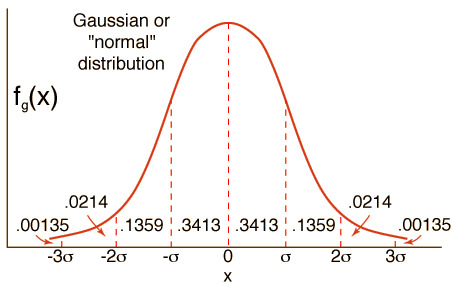
\includegraphics[scale=0.45,left]{gaussian.jpg}

    This diagram represents a single variable with a Gaussian distribution. If, for a particular domain, there existed some infinitely large number of variables, where not only does every single one fit a Gaussian distribution, but any \textit{linear} combination of all variables also fit a Gaussian distribution We can see that this is useful by first considering that in some arbitrarily large feature space, we only have a limited number of datapoints (as opposed to some infinite number presenting all data possible in a domain, which would remove the need for machine learning in any case, as we would then be able to deduce the function which described the entire dataset) - for which the \lq impossible \rq full dataset is represented by some function $f(x)$. If we then try to infer properties of the Gaussian Process by querying only on the data points that we have, the resulting properties would be the same as if we queried the true function itself, using only the same finite set of points. In summary, this means that Gaussian Processes can be used to represent data without needing to force a particular family of functions, e.g. linear functions, to be able to make predictions. ~\citep{rasmussen06}.

    \subsection{Kernel Function} In machine learning, kernels essentially define the similarity between datapoints - in other words, the function that governs the elements of the covariance matrix, which is an $n \textrm{x} n$ matrix representing the \lq similarity \rq between every point with every other point, where the element $k_{ij}$ at the coordinate $(i,j)$ of the matrix represents how \lq similar \rq those two points are as stated by the kernel. The kernel that we will be using is the squared exponential $$ k_{(x, x')} = \sigma^2 exp\left(-\frac{(x-x')^2}{2l^2}\right) + \sigma^2_{noise}I$$ where $l$, the lengthscale, describes the \textit{smoothness} of the function, and can be tuned as desired.

    \subsection{Gaussian Process Regression} From the above description, we can see that GPs do not inherently support discrete labels, due to their non-Gaussian distribution - we need to first perform regression, and coerce the result of this into a form that can be used to classify inputs. To perform GP regression, consider the datapoints:
    $$ \textrm{set } a = x_1, ... , x_l, \textrm{set } b = x_{l+1}, ... , x_n $$
    $$ \textrm{and similarly for } y: y_1, ... , y_l, y_{l+1}, ... , y_n $$
    where the former group represent data for which we do not have the corresponding ($y$) values, the latter group represents the finite amount of data and corresponding values we \textit{do} have. We then state that all these datapoints exist in some Gaussian Process $$ (Z_x) = GP(\mu, K) $$ on a set $S$ of all possible data. To perform inference on \lq unknown \rq data points using known ones, we want to get the posterior predictive distribution on $y_1, ... , y_l$ given $y_{l+1}, ... , y_n$. Note that the $y$ values are a function of points in our GP $Z$ such that $$y_i = \widetilde{Z}_x + \epsilon_i$$ where $\widetilde{Z}$ is the \lq trivial \rq case of our GP in the finite space for which we have data, and $$\epsilon = (\epsilon_i, ... , \epsilon_n) \ \textrm{for all} \ x = (x_i, ... , x_n)$$ and $\epsilon \sim N(0, \sigma^2I)$ i.e. the errors have Gaussian distribution with mean 0, and diagonal covariance matrix $\sigma^2I$. We can now define that $$\widetilde{\mu}_{a} = \widetilde{\mu}_{1} ,..., \widetilde{\mu}_{l} \textrm{ and } \widetilde{\mu}_{b} = \widetilde{\mu}_{l+1} ,..., \widetilde{\mu}_{n}$$ 
    $$ K = k_{ij} \textrm{, where } k_{ij} = k(x_i, x_j) $$
    $k$ being our kernel from our Gaussian Process $Z$. 

    We then get the covariance matrix for our known dataset and the unknown for which we want to determine the posterior predictive distribution:
    $$ K = 
    \begin{bmatrix}
        K_{aa} & K_{ab} \\
        K_{ba} & K_{bb} 
    \end{bmatrix}
    $$

    Now, we can solve for $$(Y_a | Y_b = y_b) \sim N(m, D)$$
    where $y_b$ is the aforementioned known set $y_b = (y_{l+1}, ... , y_{n})$, and $Y_a$ are our unknowns, by using the derived values of $m$ and $D$:

    $$ m = \mu_a + K_{ab} (K_{bb} + \sigma^2I)^{-1} (y_b - \mu_b) $$
    $$ D = (K_{aa} + \sigma^2I) - K_{ab} (K_{bb}+\sigma^2I)^{-1} K_{ba} $$

    The result of this posterior predictive distribution is that we can now obtain a \textit{distribution} of functions and the correctness likelihood of each, which can be visualised as below:
    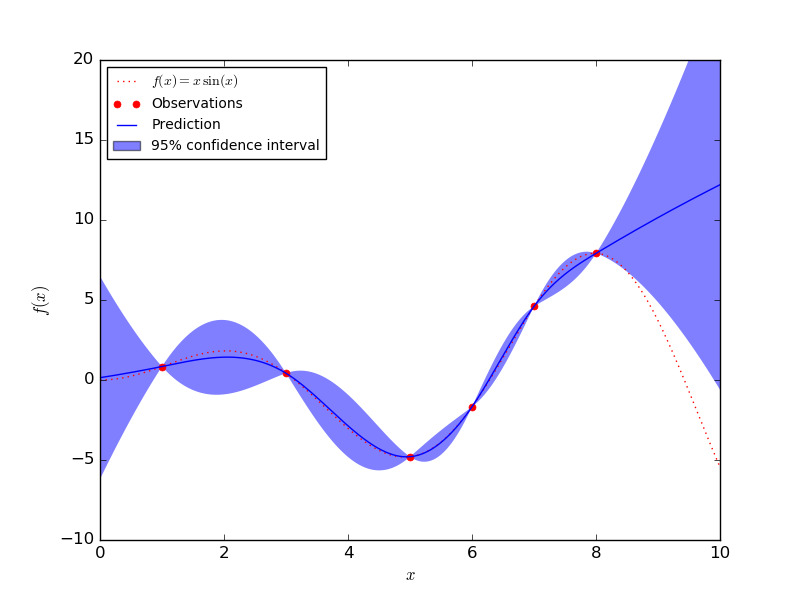
\includegraphics[scale=0.45,left]{gp-inference.jpg}

    \subsection{Gaussian Process Classification} 
    To perform Gaussian Process classification, we consider the \lq one vs all \rq (OvA) approach where we build $n$ ($n$ being the number of distinct classes) binary classifiers, where the probabilities across all the $n$ classes are combined to allow decisions to be made regarding the decided label for a particular datapoint. However, each of the individual classifiers with only binary $(0, 1)$ labels do not have Gaussian distribution, requiring some form of approximation to integrate over non-Gaussian values to obtain the estimated Gaussians. To do this, we employ the method of expectation propagation as providing the most accurate posteriors compared to other alternatives ~\citep{nickisch08}. 

    To allow GP classification, we need to first map the binary \lq labels\rq ($(0, 1)$'s) onto a continuous sigmoid function so that class membership probability can be represented as a value between $0$ and $1$. This is done using the logit function $$sig_{logit}(t) = \frac{1}{1+e^{-t}}$$
    
    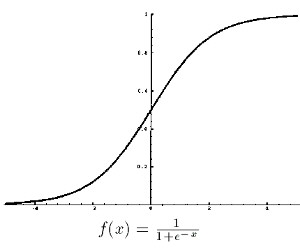
\includegraphics[scale=0.45,left]{logit.jpg}

    \subsection{Sparse Gaussian Proccess Approximation} However, there is an inherit limitation in the naive use of Gaussian proceses in that its computational complexity is $O(n^3)$ due to the covariance matrix inversion step - meaning that even our relatively 'small' training dataset of 16,000 data points is already computationally intractable ($O(4,000,000,000,000)$) without taking steps to reduce this computational requirement.

%     However, there is an inherit limitation in the use of Gaussian processes in that its computational complexity is $O(n^3)$ - meaning that for our relatively 'small' training dataset of 16,000, naive use of GPs are already computationally infeasible - let alone our unclassified dataset of 7 million (for which we wish to create a habitat map for) that only posesses corresponding low resolution (acoustic) data.
% 
% To explain Gaussian processes in simple terms - first consider a single variable that fits a Gaussian distribution, commonly known as the bell curve, or normal distribution. If we generalise this single dimension to infinitely many, where any linear combination of components is normally distributed, then this is what we call a Gaussian Process.
% 
% Compared to more commonly used supervised classification algorithms which require modeling around the chosen features, Gaussian processes instead look at the joint distribution across all features. However, they require a matrix inversion step with $O(n^3)$ complexity - this does not scale well beyond at most several thousand datapoints. To overcome this and be able to utilise as much of the available data as possible, we use approximation methods.
% 
% While a number of studies have undertaken comparing techniques in sparse GP regression, there are fewer for classification, as the stochastic nature of labels inherently steers away from being Gaussian itself. The two differ in implementation whereby in classification, the function that is otherwise used in regression has to pass its predictions through a squashing function to bound the results between (0,1), resulting in a non-Gaussian distribution. A study by ~\citet{kuss05} found that Expectation Propagation was superior to the previously used Laplace's method for projecting classes back to an approximated Gaussian distribution. It is using Expectation Propagation that we will be able to use approximated sparse GP regression techniques and apply them to classification.

\newpage
\section{Results}
\textit{(1 page)}
To compare the performance of our Gaussian Process (GP) classifier using varying sparse approximate GP methods, we want to obtain benchmarks by getting the F-scores and accuracies using deterministic machine learning algorithms. The first table represents the original 24 granular classes, whereas the second one is using the 5 aggregated classes, which are a summarisation of the more specific 24. This was done in collaboration with an expert who grouped the original unsupervised clusterings of habitat classes into similar groups, where the aggregated classes provide an obvious advantage in performance.
    
24 Habitat classes

\begin{tabular}{| l | l | l |}
    \hline
    Algorithm           & F1 score & Accuracy \\\hline
    KNN (5)             & 0.33278 & 0.62459 \\
    Logistic Regression & 0.20285 & 0.682705 \\
    Random Forest       & 0.20283 & 0.68258 \\
    SVM                 & 0.20284 & 0.68270 \\\hline
\end{tabular}

5 Aggregated habitat classes

\begin{tabular}{| l | l | l |}
    \hline
    Algorithm           & F1 score & Accuracy \\\hline
    KNN (5)             & 0.61347 & 0.749214 \\
    Logistic Regression & 0.50381 & 0.814503 \\
    Random Forest       & 0.50932 & 0.819253 \\
    SVM                 & 0.50290 & 0.818273 \\\hline
\end{tabular}

These next two set of results are using Gaussian processes with the granular and aggregated habitat classes, respectively, with different methods applied to minimise the original $O(n^3)$ computational complexity as much as possible. With the exception of the subset of data (SoD) benchmark, the rest are wrapped with Expectation Propagation

24 Habitat classes 

\begin{tabular}{| l | l | l |}
    \hline
    Approximation method    & F1 score & Accuracy \\\hline
    Subset of Data          & 0.72948 & 0.84106 \\
    SR                      & 0.79258 & 0.87151 \\
    PP                      & 0.81755 & 0.89162 \\
    FIC                     & 0.83291 & 0.91418 \\
    \hline
\end{tabular}

5 Aggregated habitat classes

\begin{tabular}{|l | l | l|}
    \hline
    Approximation method    & F1 score & Accuracy \\\hline
    Subset of Data          & 0.84281 & 0.91968 \\
    SR                      & 0.88954 & 0.93014 \\
    PP                      & 0.91758 & 0.95417 \\
    FIC                     & 0.92856 & 0.96281 \\
    \hline
\end{tabular}

Key:\\
SR - subset of regressors ; FIC - fully independent conditional ; PP - projected process

\section{Analysis, Discussion}
Approximated sparse Gaussian Processes were used to classify benthic habitats into habitat classes, and a number of ways in which to perform the approximation were tested. All of them were found to perform considerably better than the more popular and widely used methods of SVMs, Random Forests, Logistic Regression, and kNN. Of the approximation techniques, fully independent conditionaals (FITC) performed the best.

The first thing to take note of is the performance of the algorithms when classifying the aggregated classes, compared to the more granular ones. Although the reason is fairly obvious, it is worth pointing out that this is due to the variational dirichlet processes generating habitat classes that are very similar (in expert opinion) - and once consolidated, better represented the segregation subject matter experts would deem more appropriate.

Another interesting point is that in ~\citet{bender12}, only subset of data is used in their probabilistic least target squares classification, similarly using approximated Gaussian Processes, and yet achieved over 98\% accuracy. Given the distribution of data and habitat boundaries in the dataset between the two studies, Scott Reef and O'Hara Bluff respectively, the former has less distinct boundaries, with different habitats overlapping with the next quite often, whereas O'Hara Bluff has a wider variety of unique and distinct habitats from their adjacent ones, with clearer boundaries.

Moreover, (\textbf{TODO insert here}) has found that different techniques have worked better on certain datasets. Thus, to get a more comprehensive performance review of the techniques epxlored in this paper, a range of datasets from entirely different habitats need to be analysed in order to get a more holistic picture on how the tested techniques work in the arena of benthic habitat mapping in general.

\vfill
\columnbreak

\section{Conclusion \& Future Work}
\textit{(0.5 column = 0.25 page)}

Moreover, because the high resolution data used were images collected using automated vehicles that were then pre-clustered in ~\citet{steinberg11} using Variational Dirichlet Processes, the classifications themselves are also represented as continuous probabilities.

\section{References}

\bibliographystyle{plainnat}

\bibliography{Bibliography}

\end{multicols}{2}

\end{document}
